Dựa trên nền tảng lý thuyết đã xây dựng, chương này tập trung phân tích thuật toán Deutsch--Jozsa~\cite{ref2} nhằm làm rõ ưu thế tuyệt đối của tính toán lượng tử so với máy tính cổ điển. Cấu trúc của chương gồm bốn phần: mục~\ref{sec:dj-problem} xây dựng bài toán và mô hình oracle; mục 3.2 phân tích toán học thuật toán; mục 3.3 định lượng ưu thế lượng tử; và mục 3.4 cuối cùng nhằm kiểm chứng lý thuyết qua mô phỏng số với Qiskit. Nội dung phân tích thuật toán trong chương được tham khảo từ các công trình đặt nền móng của Deutsch~\cite{ref1}, Deutsch \& Jozsa~\cite{ref2}, cùng với hệ thống tài liệu hướng dẫn lập trình và thực hành mạch lượng tử trực tuyến của thư viện Qiskit.
 
\section{Phát biểu bài toán và mô hình oracle lượng tử}
\label{sec:dj-problem}
 

Thuật toán Deutsch--Jozsa được xây dựng để giải một lớp bài toán cụ thể về hàm
boolean. Mục này lần lượt giới thiệu lớp bài toán đó, mô hình oracle lượng tử
mã hóa hàm vào mạch, và cơ chế phase kickback -- ba thành phần lý thuyết quan trọng để phân tích thuật toán.

%────────────────────────────────────────────────────────────────────────────
\subsection*{Hàm boolean: constant và balanced}
%────────────────────────────────────────────────────────────────────────────

\begin{definition}[Hàm boolean $n$ bit]
Cho $n \in \mathbb{N}^*$. Một \textbf{hàm boolean $n$ bit} là ánh xạ
$$f \colon \{0,1\}^n \longrightarrow \{0,1\}.$$
Miền xác định $\{0,1\}^n$ có $N = 2^n$ phần tử, mỗi phần tử là một chuỗi
nhị phân độ dài $n$.
\end{definition}

\begin{definition}[Hàm hằng và hàm cân bằng]
\label{def:const-balanced}
Hàm $f \colon \{0,1\}^n \to \{0,1\}$ được gọi là:
\begin{enumerate}[label=(\roman*)]
    \item \textbf{Hằng} (\textit{constant}) nếu $f(x) = c$ với mọi
          $x \in \{0,1\}^n$, trong đó $c \in \{0,1\}$ là một hằng số cố định;
    \item \textbf{Cân bằng} (\textit{balanced}) nếu $f$ nhận giá trị $0$ trên
          đúng một nửa miền xác định và giá trị $1$ trên nửa còn lại:
          $$\bigl|\{x \in \{0,1\}^n : f(x)=0\}\bigr|
            = \bigl|\{x \in \{0,1\}^n : f(x)=1\}\bigr| = 2^{n-1}.$$
\end{enumerate}
\end{definition}

\begin{example}[Minh họa với $n=2$]
\label{ex:const-balanced-n2}
Với $n=2$, miền xác định là $\{00, 01, 10, 11\}$ gồm $4$ phần tử.
\begin{itemize}
    \item Hàm hằng: $f_0(x) = 0$ với mọi $x$ (hoặc $f_1(x) = 1$ với mọi $x$).
    \item Hàm cân bằng: chẳng hạn $f(00)=f(01)=0$ và $f(10)=f(11)=1$ --
          đúng $2$ đầu vào cho ra $0$ và $2$ đầu vào cho ra $1$.
\end{itemize}

\end{example}

\begin{remark}
Hai lớp hàm hằng và cân bằng là rời nhau. Với $n \geq 1$, số hàm hằng luôn
là $2$, trong khi số hàm cân bằng là $\binom{2^n}{2^{n-1}}$, tăng rất nhanh
theo $n$. Chẳng hạn với $n=3$, có $\binom{8}{4} = 70$ hàm cân bằng nhưng
chỉ có $2$ hàm hằng.
\end{remark}

%────────────────────────────────────────────────────────────────────────────
\subsection*{Bài toán Deutsch ($n=1$) và tổng quát hóa $n$ bit}
%────────────────────────────────────────────────────────────────────────────

Năm 1985, D.\ Deutsch \cite{ref1} đặt ra câu hỏi: liệu một máy tính lượng tử
có thể xác định tính chất \emph{toàn cục} của một hàm boolean bằng ít lần truy
vấn hơn máy tính cổ điển không? Câu hỏi này dẫn đến phiên bản đơn giản nhất
của bài toán.

\begin{definition}[Bài toán Deutsch]
\label{def:deutsch-problem}
Cho một hàm $f \colon \{0,1\} \to \{0,1\}$ được cung cấp dưới dạng
\textbf{hộp đen} (\textit{black box}): chỉ có thể truy vấn giá trị $f(x)$ tại
các điểm $x$, không thể kiểm tra cấu trúc bên trong của $f$. Bài toán yêu cầu
xác định $f$ là hằng hay cân bằng.
\end{definition}

\begin{remark}
Với $n=1$, chỉ có bốn hàm boolean: hai hàm hằng ($f \equiv 0$ và $f \equiv 1$)
và hai hàm cân bằng ($f = \mathrm{id}$ tức $f(x)=x$, và $f = \mathrm{NOT}$ tức
$f(x)=1-x$). Một thuật toán cổ điển tất định cần tối thiểu $2$ lần truy vấn để
phân biệt hai lớp này -- vì một lần truy vấn duy nhất chỉ tiết lộ $f(0)$ hoặc
$f(1)$, không đủ để kết luận. Thuật toán Deutsch \cite{ref1} giải quyết bài toán
chỉ với \emph{một} lần truy vấn oracle lượng tử.
\end{remark}

Năm 1992, Deutsch và Jozsa \cite{ref2} tổng quát hóa bài toán lên $n$ bit tùy ý.

\begin{definition}[Bài toán Deutsch--Jozsa]
\label{def:dj-problem}
Cho $n \in \mathbb{N}^*$ và một hàm $f \colon \{0,1\}^n \to \{0,1\}$ được
\emph{đảm bảo} (\textit{promise}) thuộc một trong hai lớp hàm hằng hoặc hàm cân bằng. Bài toán yêu cầu xác định $f$ là hằng hay cân
bằng, với $f$ được truy cập thông qua một oracle lượng tử.
\end{definition}

\begin{remark}
Điều kiện ``được đảm bảo'' là bản chất của bài toán: không có giả thiết này,
không tồn tại thuật toán nào -- cổ điển hay lượng tử -- có thể đưa ra câu trả
lời đúng trong mọi trường hợp mà không truy vấn hết miền xác định. Trong trường
hợp cổ điển tất định, cần tối thiểu $2^{n-1}+1$ lần truy vấn để đảm bảo kết
quả chính xác \cite{ref5}: nếu $2^{n-1}$ lần truy vấn đầu cho cùng một giá trị,
$f$ vẫn có thể là hằng \emph{hoặc} cân bằng cho đến khi thực hiện thêm ít nhất
một lần truy vấn nữa. Thuật toán Deutsch--Jozsa giải quyết bài toán chỉ với
\emph{một} lần truy vấn oracle.
\end{remark}



%────────────────────────────────────────────────────────────────────────────
\subsection*{Toán tử oracle $U_f$ và phase kickback}
%────────────────────────────────────────────────────────────────────────────

Để tích hợp hàm $f$ vào mạch lượng tử, cần một biểu diễn toán tử unitary của
$f$. Theo Tiên đề~2 (mục~\ref{sec:postulates}), mọi phép biến đổi lượng tử đều
phải là unitary -- và do đó khả nghịch. Tuy nhiên, phần lớn các hàm boolean
không khả nghịch: nhiều đầu vào có thể cho cùng đầu ra, khiến không thể phục hồi
$x$ từ $f(x)$. Để giải quyết mâu thuẫn này, ta mở rộng không gian trạng thái
bằng cách thêm một \textbf{qubit phụ} (\textit{ancilla qubit}).

\begin{definition}[Oracle lượng tử $U_f$]
\label{def:oracle}
Cho $f \colon \{0,1\}^n \to \{0,1\}$. \textbf{Oracle lượng tử} $U_f$ là toán
tử unitary tác động trên không gian $(\mathbb{C}^2)^{\otimes n} \otimes
\mathbb{C}^2$ theo quy tắc:
$$U_f \colon |x\rangle|y\rangle \;\longmapsto\; |x\rangle|y \oplus f(x)\rangle,$$
trong đó $x \in \{0,1\}^n$, $y \in \{0,1\}$, và $\oplus$ là phép cộng modulo $2$.
Thanh ghi $|x\rangle$ ($n$ qubit) được gọi là \textbf{thanh ghi vào}; qubit
$|y\rangle$ được gọi là \textbf{qubit đích} (\textit{target qubit}).
\end{definition}


\begin{figure}[H]
    \centering
    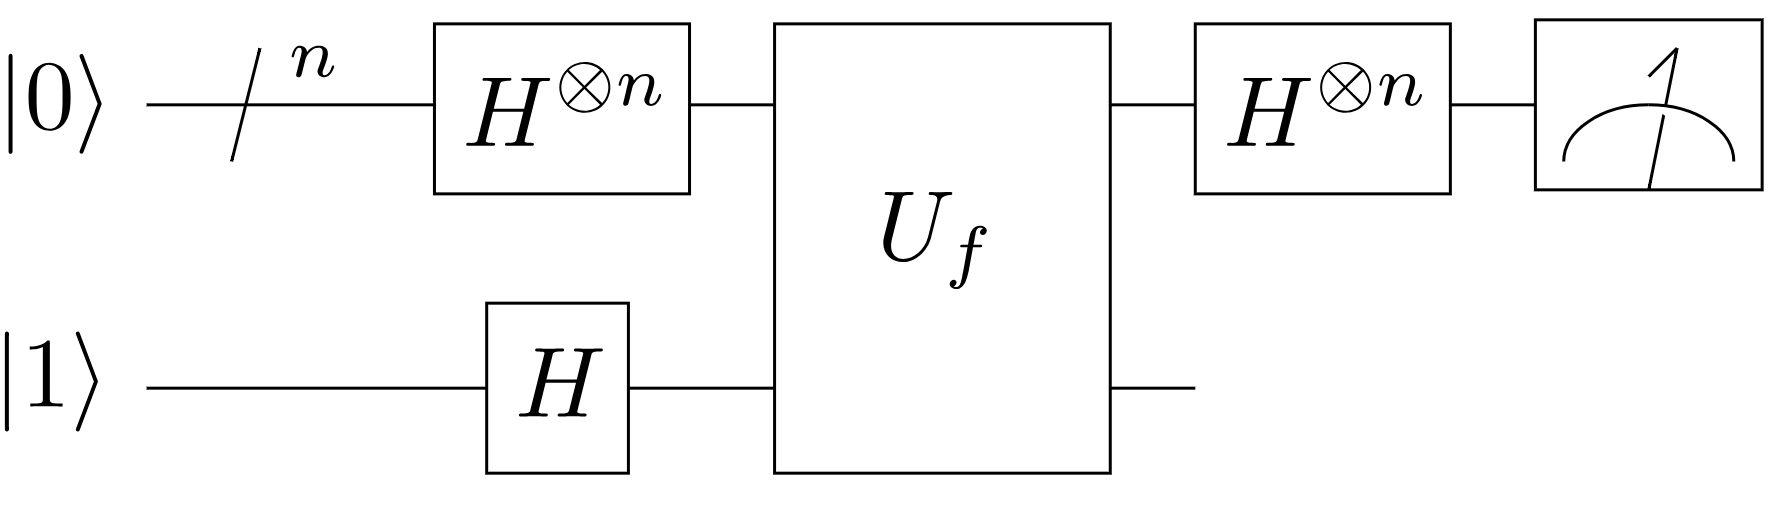
\includegraphics[width=0.8\textwidth]{assets/machDJ.png}
    \caption{Minh họa biểu đồ có chứa mạch oracle $U_f$.}
\end{figure}

\begin{proposition}
\label{prop:uf-unitary}
Toán tử $U_f$ là toán tử unitary và tự nghịch đảo ($U_f^2 = I$).
\end{proposition}

\begin{proof}
$U_f$ hoán vị các phần tử của cơ sở tính toán $\{|x\rangle|y\rangle\}$ vì với
mọi $x, y$: $y \oplus f(x) \oplus f(x) = y$. Hoán vị bảo toàn tích trong nên
$U_f$ là unitary. Áp dụng $U_f$ hai lần:
$$U_f^2|x\rangle|y\rangle
= U_f|x\rangle|y \oplus f(x)\rangle
= |x\rangle|y \oplus f(x) \oplus f(x)\rangle
= |x\rangle|y\rangle.$$
Vậy $U_f^2 = I$, tức $U_f^{-1} = U_f = U_f^\dagger$.
\end{proof}

\begin{remark}
Tính chất $U_f^2 = I$ -- tự nghịch đảo -- là hệ quả trực tiếp của phép cộng
modulo $2$: áp dụng oracle hai lần khôi phục lại trạng thái ban đầu. Đây cũng
là lý do thiết kế oracle theo cấu trúc $|x\rangle|y \oplus f(x)\rangle$ thay vì
lưu trực tiếp $f(x)$ vào một qubit: cấu trúc này đảm bảo tính khả nghịch mà
không cần thêm bước xóa bộ nhớ.
\end{remark}

Cơ chế quan trọng nhất quyết định hiệu quả của thuật toán là \textbf{phase
kickback}: thay vì đọc kết quả từ qubit đích, ta chuẩn bị qubit đích ở trạng
thái đặc biệt sao cho thông tin về $f(x)$ được ``đẩy ngược'' vào pha của thanh
ghi vào.

\begin{proposition}[Phase kickback]
\label{prop:phase-kickback}
Nếu qubit đích được chuẩn bị ở trạng thái
$|{-}\rangle = \dfrac{|0\rangle - |1\rangle}{\sqrt{2}}$, thì:
$$U_f\bigl(|x\rangle \otimes |{-}\rangle\bigr)
= (-1)^{f(x)}\,|x\rangle \otimes |{-}\rangle.$$
\end{proposition}

\begin{proof}
Khai triển $|{-}\rangle$ và áp dụng tuyến tính:
\begin{align*}
U_f\!\left(|x\rangle \otimes \frac{|0\rangle - |1\rangle}{\sqrt{2}}\right)
&= \frac{1}{\sqrt{2}}\Bigl(
    U_f|x\rangle|0\rangle - U_f|x\rangle|1\rangle
  \Bigr) \\
&= \frac{1}{\sqrt{2}}\Bigl(
    |x\rangle|f(x)\rangle - |x\rangle|1 \oplus f(x)\rangle
  \Bigr).
\end{align*}

\noindent\textbf{Trường hợp $f(x)=0$:}
$$= \frac{1}{\sqrt{2}}\bigl(|x\rangle|0\rangle - |x\rangle|1\rangle\bigr)
= |x\rangle \otimes |{-}\rangle = (-1)^0\,|x\rangle \otimes |{-}\rangle.$$

\noindent\textbf{Trường hợp $f(x)=1$:}
$$= \frac{1}{\sqrt{2}}\bigl(|x\rangle|1\rangle - |x\rangle|0\rangle\bigr)
= -|x\rangle \otimes |{-}\rangle = (-1)^1\,|x\rangle \otimes |{-}\rangle.$$

Gộp hai trường hợp: $U_f(|x\rangle \otimes |{-}\rangle)
= (-1)^{f(x)}|x\rangle \otimes |{-}\rangle$.
\end{proof}

\begin{remark}
Mệnh đề~\ref{prop:phase-kickback} có ba hệ quả quan trọng cần lưu ý.

\textbf{Thứ nhất}, qubit đích \emph{không thay đổi} sau tác động của $U_f$: nó
vẫn ở trạng thái $|{-}\rangle$ bất kể giá trị $f(x)$. Điều này giải thích tên
gọi ``phase kickback'': pha $(-1)^{f(x)}$ bị ``đá ngược'' từ qubit đích lên
thanh ghi vào, thay vì lưu lại ở qubit đích.

\textbf{Thứ hai}, pha $(-1)^{f(x)}$ là pha \emph{toàn cục} khi xét trên một
trạng thái đơn lẻ $|x\rangle$ -- không thể đo trực tiếp. Tuy nhiên, khi thanh ghi vào ở trạng thái
\emph{chồng chất} $\sum_x \alpha_x|x\rangle$, pha $(-1)^{f(x)}$ trở thành pha
\emph{tương đối} giữa các số hạng -- và do đó có thể quan sát được qua giao
thoa lượng tử.

\textbf{Thứ ba}, đây là lý do qubit đích được gọi là \emph{qubit phụ} theo
nghĩa chức năng: sau khi đóng vai trò trung gian truyền thông tin từ pha
thanh ghi vào, nó không tham gia vào phép đo cuối mạch.
\end{remark}

\begin{remark}
Cơ chế phase kickback không đặc thù cho thuật toán Deutsch--Jozsa mà là một
kỹ thuật tổng quát, xuất hiện trong nhiều thuật toán lượng tử quan trọng như
thuật toán Grover (tìm kiếm) và thuật toán Shor (phân tích nhân tử). Nielsen
và Chuang \cite{ref5} coi đây là một trong những kỹ thuật nền tảng của lập
trình lượng tử.
\end{remark}



\section{Phân tích toán học từng bước thuật toán}
Mục này trình bày phân tích toán học đầy đủ thuật toán Deutsch--Jozsa cho hàm
$f:\{0,1\}^n \to \{0,1\}$, theo từng bước biến đổi trạng thái bằng ký hiệu
Dirac. Ký hiệu $|x\rangle$ với $x \in \{0,1\}^n$ chỉ trạng thái cơ sở tính
toán của $n$ qubit đầu vào, và phép đo ở bước cuối được phân tích theo Tiên
đề~3 (mục~\ref{sec:postulates}).
 
% ---------------------------------------------------------------
\subsection*{Bước 1: Chuẩn bị trạng thái ban đầu}
 
Hệ gồm $n+1$ qubit được khởi tạo ở trạng thái:
\begin{equation}
    |\psi_0\rangle = |0\rangle^{\otimes n}|1\rangle.
    \label{eq:dj-init}
\end{equation}
$n$ qubit đầu tiên (thanh ghi đầu vào) ở trạng thái $|0\rangle^{\otimes n}$,
qubit thứ $(n+1)$ (qubit bổ trợ, \textit{ancilla}) ở trạng thái $|1\rangle$.
Việc chọn $|1\rangle$ cho qubit bổ trợ -- thay vì $|0\rangle$ -- là điều kiện
cần thiết để cơ chế \textit{phase kickback} hoạt động ở Bước~3, như sẽ thấy
rõ bên dưới.
 
% ---------------------------------------------------------------
\subsection*{Bước 2: Biến đổi Hadamard $H^{\otimes(n+1)}$}
 
Áp dụng cổng Hadamard đồng thời lên tất cả $n+1$ qubit. Sử dụng kết quả
$H|0\rangle = |{+}\rangle$ và $H|1\rangle = |{-}\rangle$,
trạng thái sau biến đổi là:
\begin{equation}
    |\psi_1\rangle
    = H^{\otimes n}|0\rangle^{\otimes n} \otimes H|1\rangle
    = \frac{1}{\sqrt{2^n}}\sum_{x=0}^{2^n-1}|x\rangle
      \otimes \frac{|0\rangle - |1\rangle}{\sqrt{2}}.
    \label{eq:dj-hadamard1}
\end{equation}
Thanh ghi đầu vào đạt trạng thái chồng chất đồng đều trên tất cả $2^n$ chuỗi
bit -- đây là biểu thức~\eqref{eq:uniform-superposition} đã giới thiệu ở
mục~\ref{sec:qubit}. Qubit bổ trợ ở trạng thái $|{-}\rangle =
\frac{|0\rangle-|1\rangle}{\sqrt{2}}$, trạng thái sẽ hấp thụ thông tin về
$f$ dưới dạng pha ở bước tiếp theo.
 
% ---------------------------------------------------------------
\subsection*{Bước 3 \quad Áp dụng oracle $U_f$ và phase kickback}
 
Oracle $U_f$ tác động lên toàn hệ theo quy tắc
$U_f|x\rangle|y\rangle = |x\rangle|y \oplus f(x)\rangle$. Tác động lên từng hạng tử của~\eqref{eq:dj-hadamard1},
xét riêng qubit bổ trợ ở trạng thái $\frac{|0\rangle-|1\rangle}{\sqrt{2}}$:
 
\begin{itemize}
    \item Nếu $f(x) = 0$: $U_f|x\rangle\frac{|0\rangle-|1\rangle}{\sqrt{2}}
          = |x\rangle\frac{|0\rangle-|1\rangle}{\sqrt{2}}
          = (+1)\cdot|x\rangle\frac{|0\rangle-|1\rangle}{\sqrt{2}}.$
    \item Nếu $f(x) = 1$: $U_f|x\rangle\frac{|0\rangle-|1\rangle}{\sqrt{2}}
          = |x\rangle\frac{|1\rangle-|0\rangle}{\sqrt{2}}
          = (-1)\cdot|x\rangle\frac{|0\rangle-|1\rangle}{\sqrt{2}}.$
\end{itemize}
 
Trong cả hai trường hợp, qubit bổ trợ \emph{trở lại} trạng thái
$\frac{|0\rangle-|1\rangle}{\sqrt{2}}$ (không bị thay đổi), còn toàn bộ thông
tin về $f(x)$ được \emph{đẩy ngược} vào pha của thanh ghi đầu vào dưới dạng
hệ số $(-1)^{f(x)}$ -- đây chính là cơ chế \textbf{phase kickback}. Hai trường
hợp gộp lại thành:
\begin{equation}
    U_f\left(|x\rangle\frac{|0\rangle-|1\rangle}{\sqrt{2}}\right)
    = (-1)^{f(x)}|x\rangle\frac{|0\rangle-|1\rangle}{\sqrt{2}}.
    \label{eq:kickback}
\end{equation}
Áp dụng~\eqref{eq:kickback} cho toàn bộ trạng thái~\eqref{eq:dj-hadamard1},
qubit bổ trợ tách ra như một thừa số chung và từ đây có thể bỏ qua:
\begin{equation}
    |\psi_2\rangle
    = \frac{1}{\sqrt{2^n}}\sum_{x=0}^{2^n-1}(-1)^{f(x)}|x\rangle
      \otimes \frac{|0\rangle-|1\rangle}{\sqrt{2}}.
    \label{eq:dj-after-oracle}
\end{equation}
 
% ---------------------------------------------------------------
\subsection*{Bước 4 \quad Hadamard lần hai và xác suất đo}
 
\subsubsection*{Biến đổi Hadamard lần hai}
 
Áp dụng $H^{\otimes n}$ lên thanh ghi đầu vào. Sử dụng công thức tổng quát
của biến đổi Hadamard trên $n$ qubit \cite{ref5}:
\begin{equation}
    H^{\otimes n}|x\rangle
    = \frac{1}{\sqrt{2^n}}\sum_{z=0}^{2^n-1}(-1)^{x\cdot z}|z\rangle,
    \label{eq:hadamard-general}
\end{equation}
trong đó $x \cdot z = \sum_{k=1}^{n} x_k z_k \pmod{2}$ là tích vô hướng bit.
Thay~\eqref{eq:hadamard-general} vào~\eqref{eq:dj-after-oracle}:
\begin{align}
    |\psi_3\rangle
    &= \frac{1}{\sqrt{2^n}}\sum_{x=0}^{2^n-1}(-1)^{f(x)}
       \cdot\frac{1}{\sqrt{2^n}}\sum_{z=0}^{2^n-1}(-1)^{x\cdot z}|z\rangle
       \notag\\
    &= \sum_{z=0}^{2^n-1}
       \left(\frac{1}{2^n}\sum_{x=0}^{2^n-1}(-1)^{f(x)+x\cdot z}\right)|z\rangle.
    \label{eq:dj-final}
\end{align}
 
\subsubsection*{Tính xác suất đo trạng thái $|0\rangle^{\otimes n}$}
 
Theo Hệ quả~\ref{cor:born} (Quy tắc Born), biên độ xác suất đo được
$|0\rangle^{\otimes n}$ (tức $z = 0$) là hệ số đứng trước $|0\rangle^{\otimes n}$
trong~\eqref{eq:dj-final}:
\begin{equation}
    A_0 = \frac{1}{2^n}\sum_{x=0}^{2^n-1}(-1)^{f(x)},
    \label{eq:amplitude-zero}
\end{equation}
và xác suất đo được $|0\rangle^{\otimes n}$ là $p(0^n) = |A_0|^2$.
 
\begin{proposition}[Tiêu chuẩn phân loại Deutsch--Jozsa]
\label{prop:dj-criterion}
Với hàm $f:\{0,1\}^n\to\{0,1\}$ là hằng số hoặc cân bằng:
\begin{enumerate}[label=(\roman*)]
    \item Nếu $f$ \textbf{hằng số}: $f(x) = c$ với mọi $x$, nên
          $(-1)^{f(x)} = (-1)^c = \pm 1$ không đổi. Tổng~\eqref{eq:amplitude-zero}
          là $2^n$ số hạng cùng dấu:
          $$A_0 = \frac{1}{2^n}\cdot 2^n\cdot(\pm 1) = \pm 1,$$
          do đó $p(0^n) = |A_0|^2 = 1$. Phép đo \emph{luôn} cho kết quả
          $|0\rangle^{\otimes n}$.
    \item Nếu $f$ \textbf{cân bằng}: đúng $2^{n-1}$ giá trị $x$ cho
          $(-1)^{f(x)} = +1$ và $2^{n-1}$ giá trị cho $(-1)^{f(x)} = -1$,
          các số hạng triệt tiêu nhau hoàn toàn:
          $$A_0 = \frac{1}{2^n}\cdot(2^{n-1} - 2^{n-1}) = 0,$$
          do đó $p(0^n) = 0$. Phép đo \emph{không bao giờ} cho kết quả
          $|0\rangle^{\otimes n}$.
\end{enumerate}
\end{proposition}
 
\begin{remark}
Mệnh đề~\ref{prop:dj-criterion} cho thấy hai trường hợp hoàn toàn phân biệt
nhau: xác suất nhận giá trị $1$ hoặc $0$, không có vùng trung gian. Vì vậy,
\emph{một lần} áp dụng oracle và một lần đo là đủ để kết luận chắc chắn.
Cơ chế nền tảng là giao thoa lượng tử: ở trường hợp hằng số, các biên độ cùng
pha tăng cường lẫn nhau và tập trung hoàn toàn vào $|0\rangle^{\otimes n}$; ở
trường hợp cân bằng, các biên độ ngược pha triệt tiêu nhau hoàn toàn tại cùng
trạng thái đó.
\end{remark}

\section{Ưu thế lượng tử: $O(1)$ vs $O(2^{n-1})$}
Mục này phân tích ưu thế của thuật toán Deutsch--Jozsa so với mọi thuật toán
cổ điển tất định, phân tích vai trò của giao thoa lượng tử như cơ chế nền tảng
tạo ra ưu thế đó, và thảo luận về giới hạn cũng như ý nghĩa thực tiễn của kết
quả.
 
% ---------------------------------------------------------------
\subsection*{So sánh độ phức tạp}
 
\subsubsection*{Thuật toán lượng tử: $O(1)$ lần truy vấn oracle}
 
Toàn bộ thuật toán Deutsch--Jozsa
thực hiện đúng \textbf{một lần} truy vấn oracle $U_f$ và cho kết quả chắc chắn:
phép đo thanh ghi đầu vào sau Hadamard lần hai luôn ra $|0\rangle^{\otimes n}$
nếu $f$ hằng số, và không bao giờ ra $|0\rangle^{\otimes n}$ nếu $f$ cân bằng
(Mệnh đề~\ref{prop:dj-criterion}). Độ phức tạp truy vấn là:
\begin{equation}
    Q_{\text{lượng tử}} = 1 = O(1).
    \label{eq:quantum-complexity}
\end{equation}
 
\subsubsection*{Thuật toán cổ điển tất định: $O(2^{n-1}+1)$ lần truy vấn}
 
Một thuật toán cổ điển \emph{tất định} (\textit{deterministic}) phải truy vấn
$f$ tuần tự tại các điểm $x_1, x_2, \ldots$ cho đến khi có thể kết luận chắc
chắn. Trong trường hợp xấu nhất:
 
\begin{itemize}
    \item Sau $k < 2^{n-1}+1$ lần truy vấn, nếu tất cả đều cho cùng kết quả
          (ví dụ đều bằng $0$), thuật toán chưa thể phân biệt: $f$ có thể là
          hằng số $0$, hoặc là hàm cân bằng với đúng $2^{n-1}$ giá trị $0$ và
          $2^{n-1}$ giá trị $1$ (trong đó các điểm chưa được truy vấn đều là $1$).
    \item Chỉ sau khi truy vấn $2^{n-1}+1$ điểm và nhận được cùng kết quả, thuật
          toán mới có thể kết luận $f$ là hằng số -- vì một hàm cân bằng không
          thể có nhiều hơn $2^{n-1}$ điểm cùng giá trị.
\end{itemize}
 
Do đó độ phức tạp truy vấn trong trường hợp xấu nhất là:
\begin{equation}
    Q_{\text{cổ điển}} = 2^{n-1} + 1 = O(2^n).
    \label{eq:classical-complexity}
\end{equation}
 
\begin{remark}
Cần phân biệt \emph{độ phức tạp truy vấn} (số lần gọi oracle) và \emph{độ phức
tạp thời gian} (số cổng lượng tử). Về độ phức tạp thời gian, thuật toán
Deutsch--Jozsa cần $O(n)$ cổng Hadamard và một lần áp dụng $U_f$ -- hiệu quả
hơn đáng kể so với $O(2^n)$ bước của thuật toán cổ điển, nhưng so sánh chính
xác phụ thuộc vào cách triển khai oracle $U_f$ trên phần cứng cụ thể.
\end{remark}
 
% ---------------------------------------------------------------
\subsection*{Vai trò của giao thoa lượng tử}
 
Ưu thế $O(1)$ không đến từ tính song song lượng tử đơn thuần -- sự chồng chất
$\frac{1}{\sqrt{2^n}}\sum_x |x\rangle$ mã hóa $2^n$ đầu vào đồng thời, nhưng
phép đo ngẫu nhiên trên trạng thái này chỉ trả về một giá trị duy nhất. Ưu thế
thực sự đến từ \textbf{giao thoa lượng tử} như một cơ chế kiểm soát có chọn
lọc phân bố xác suất.
 
Nhìn lại biên độ xác suất~\eqref{eq:amplitude-zero}:
$$A_0 = \frac{1}{2^n}\sum_{x=0}^{2^n-1}(-1)^{f(x)}.$$
Đây là \emph{tổng giao thoa} của $2^n$ biên độ phức, mỗi biên độ mang pha
$(-1)^{f(x)} \in \{+1, -1\}$:
 
\begin{itemize}
    \item \textbf{Hàm hằng số -- giao thoa tăng cường:} mọi số hạng cùng dấu,
          tổng đạt giá trị cực đại $|A_0| = 1$. Toàn bộ xác suất tập trung vào
          $|0\rangle^{\otimes n}$.
    \item \textbf{Hàm cân bằng -- giao thoa triệt tiêu:} số hạng $+1$ và $-1$
          bằng nhau, tổng triệt tiêu hoàn toàn $A_0 = 0$. Xác suất đo được
          $|0\rangle^{\otimes n}$ bằng không.
\end{itemize}
 
Hai trường hợp được thiết kế để phân biệt nhau \emph{hoàn toàn} tại một điểm
duy nhất trong không gian kết quả đo -- đây là lý do một phép đo là đủ.
 
% ---------------------------------------------------------------
\subsection*{Giới hạn và ý nghĩa thực tiễn}
 
\subsubsection*{Giới hạn của bài toán}
 
Ưu thế mũ của thuật toán Deutsch--Jozsa được xây dựng trên một \textbf{giả
thiết mạnh}: đầu vào được đảm bảo là hằng số hoặc cân bằng -- không có trường
hợp nào khác. Trong thực tế, hàm $f$ tùy ý có thể không thỏa mãn điều kiện
này, và thuật toán không cung cấp cơ chế xử lý trường hợp trung gian.
 
Ngoài ra, nếu cho phép thuật toán cổ điển sử dụng \textbf{ngẫu nhiên}
(\textit{randomized algorithm}), khoảng cách về độ phức tạp thu hẹp đáng kể:
chỉ cần truy vấn $O(1)$ điểm ngẫu nhiên, thuật toán cổ điển ngẫu nhiên có thể
kết luận đúng với xác suất tùy ý gần $1$ \cite{ref5}. Cụ thể, nếu truy vấn $k$
điểm ngẫu nhiên và nhận được cùng kết quả, xác suất kết luận sai (tức $f$ thực
ra là cân bằng) không vượt quá $2^{1-k}$. Với $k = 30$, xác suất sai nhỏ hơn
$10^{-9}$ -- đủ cho hầu hết ứng dụng thực tế. Như vậy, ưu thế \emph{mũ tuyệt
đối} của thuật toán Deutsch--Jozsa chỉ tồn tại so với \emph{thuật toán cổ điển
tất định}, không phải so với thuật toán ngẫu nhiên.
 
\subsubsection*{Ý nghĩa lý thuyết}
 
Dù có giới hạn thực tiễn, thuật toán Deutsch--Jozsa mang ý nghĩa lý thuyết nền
tảng theo ba phương diện:
 
\begin{enumerate}
    \item \textbf{Bằng chứng đầu tiên về ưu thế lượng tử tất định.} Đây là
          thuật toán lượng tử đầu tiên được chứng minh \emph{chắc chắn} (không
          phải xác suất) nhanh hơn mọi thuật toán cổ điển tất định tương đương
          \cite{ref3}. Kết quả này thiết lập nguyên tắc rằng máy tính lượng tử
          có thể vượt trội máy tính cổ điển về mặt lý thuyết.
    \item \textbf{Mô hình thiết kế thuật toán lượng tử.} Cấu trúc
          khởi tạo $\to$ Hadamard $\to$ oracle $\to$ Hadamard $\to$ đo là mẫu
          thiết kế xuất hiện lại trong nhiều thuật toán lượng tử quan trọng hơn,
          bao gồm thuật toán Simon, biến đổi Fourier lượng tử, và thuật toán
          Shor \cite{ref5}.
    \item \textbf{Minh họa nguyên lý giao thoa có kiểm soát.} Thuật toán cho
          thấy rằng giá trị của tính toán lượng tử không nằm ở việc \emph{thử
          song song} $2^n$ đầu vào, mà ở việc \emph{thiết kế giao thoa} sao
          cho kết quả mong muốn được khuếch đại và kết quả không mong muốn bị
          triệt tiêu -- nguyên lý cốt lõi của hầu hết thuật toán lượng tử hiệu
          quả đã biết.
\end{enumerate}

\section{Triển khai mô phỏng với Qiskit}
\label{sec:qiskit}

Phần lý thuyết ở các mục trước đã chứng minh chặt chẽ rằng thuật toán
Deutsch--Jozsa cho kết quả đúng với xác suất $1$ trong một lần truy vấn
oracle duy nhất. Mục này hiện thực hóa
và kiểm chứng kết quả đó bằng mô phỏng số trên nền tảng Qiskit, với
$n = 1, 2, 3, 4, 5$ qubit đầu vào.

%────────────────────────────────────────────────────────────────────────────
\subsection*{Môi trường và cấu hình}
%────────────────────────────────────────────────────────────────────────────

Toàn bộ mô phỏng được thực hiện trên môi trường Python với các thư viện
chính như sau:

\begin{table}[htbp]
\centering
\caption{Môi trường phần mềm cho mô phỏng}
\label{tab:env}
\begin{tabular}{ll}
\hline
\textbf{Thành phần} & \textbf{Phiên bản} \\
\hline
Python        & 3.10 \\
Qiskit        & 1.0  \\
qiskit-aer    & 0.13 \\
NumPy         & 1.26 \\
Matplotlib    & 3.8  \\
\hline
\end{tabular}

\end{table}

Bộ mô phỏng được sử dụng là \texttt{StatevectorSimulator} của Qiskit Aer.
Toàn bộ mã nguồn được công bố trong
Phụ lục 1.

%────────────────────────────────────────────────────────────────────────────
\subsection*{Xây dựng oracle: constant và balanced}
%────────────────────────────────────────────────────────────────────────────

Để mô phỏng, cần xây dựng tường minh hai loại oracle $U_f$ tương ứng với
hàm hằng và hàm cân bằng.

\textbf{Oracle hằng.} Với hàm hằng $f \equiv c$, oracle $U_f$ tác động theo
$|x\rangle|y\rangle \mapsto |x\rangle|y \oplus c\rangle$. Điều này có nghĩa:
\begin{itemize}
    \item $f \equiv 0$: oracle là toán tử đồng nhất $I$ -- không tác động
          lên qubit nào.
    \item $f \equiv 1$: oracle chỉ áp dụng cổng $X$ lên qubit đích, độc lập
          với mọi qubit đầu vào.
\end{itemize}
Cả hai trường hợp đều không tạo ra sự vướng víu giữa thanh ghi vào và
qubit đích.

\textbf{Oracle cân bằng.} Với hàm cân bằng, chọn một chuỗi nhị phân $s \in \{0,1\}^n$ bất kỳ (không phải chuỗi
toàn $0$), đặt $f(x) = s \cdot x \pmod{2}$, và cài đặt oracle bằng các
cổng CNOT: với mỗi bit $s_j = 1$, áp dụng $\mathrm{CNOT}$ từ qubit $j$
của thanh ghi vào đến qubit đích. Hàm thu được là cân bằng vì đúng một
nửa các chuỗi $x$ thỏa mãn $s \cdot x = 0$.

\begin{example}[Oracle cân bằng với $n=2$, $s=11$]
\label{ex:oracle-balanced-n2}
Với $n=2$ và $s=11$, hàm $f(x_1 x_2) = x_1 \oplus x_2$ cho:
$f(00)=0,\; f(01)=1,\; f(10)=1,\; f(11)=0$ -- đúng hai giá trị $0$ và
hai giá trị $1$, thỏa điều kiện cân bằng. Oracle tương ứng áp dụng hai
cổng CNOT: từ $q_0$ đến $q_2$ và từ $q_1$ đến $q_2$.
\end{example}

\subsection*{Mã giả cho quá trình xây dựng và chạy mạch}

\begin{algorithm}[H]
\label{alg:dj}
\begin{algorithmic}[1]
\Require Số qubit $n$, loại oracle (\texttt{constant}/\texttt{balanced}),
         tham số $s \in \{0,1\}^n$ (nếu balanced)
\Ensure Vectơ trạng thái cuối, biểu đồ xác suất, kết luận
\State Khởi tạo mạch $n+1$ qubit, $n$ bit cổ điển
\State Áp dụng $X$ lên qubit $n$ 
\State Áp dụng $H$ lên tất cả $n+1$ qubit
\If{oracle là hằng}
    \If{$f \equiv 1$} áp dụng $X$ lên qubit $n$ \EndIf
\Else
    \For{$j = 0$ đến $n-1$}
        \If{$s_j = 1$} áp dụng $\mathrm{CNOT}(j, n)$ \EndIf
    \EndFor
\EndIf
\State Áp dụng $H$ lên qubit $0$ đến $n-1$
\State Đo qubit $0$ đến $n-1$
\State Chạy trên \texttt{StatevectorSimulator}, lấy xác suất
\If{$P(|0\rangle^{\otimes n}) = 1$} \Return \textbf{constant}
\Else{} \Return \textbf{baleanced}
\EndIf
\end{algorithmic}
\caption{Xây dựng và mô phỏng mạch Deutsch--Jozsa}
\end{algorithm}

%────────────────────────────────────────────────────────────────────────────
\subsection*{Biểu đồ xác suất và kiểm chứng $n = 1, \ldots, 5$}
%────────────────────────────────────────────────────────────────────────────

Mô phỏng được thực hiện cho $n = 1, 2, 3, 4, 5$ với cả hai loại oracle.
Hình sau minh họa kết quả cho $n=3$.


\begin{figure}[H]
    \centering
    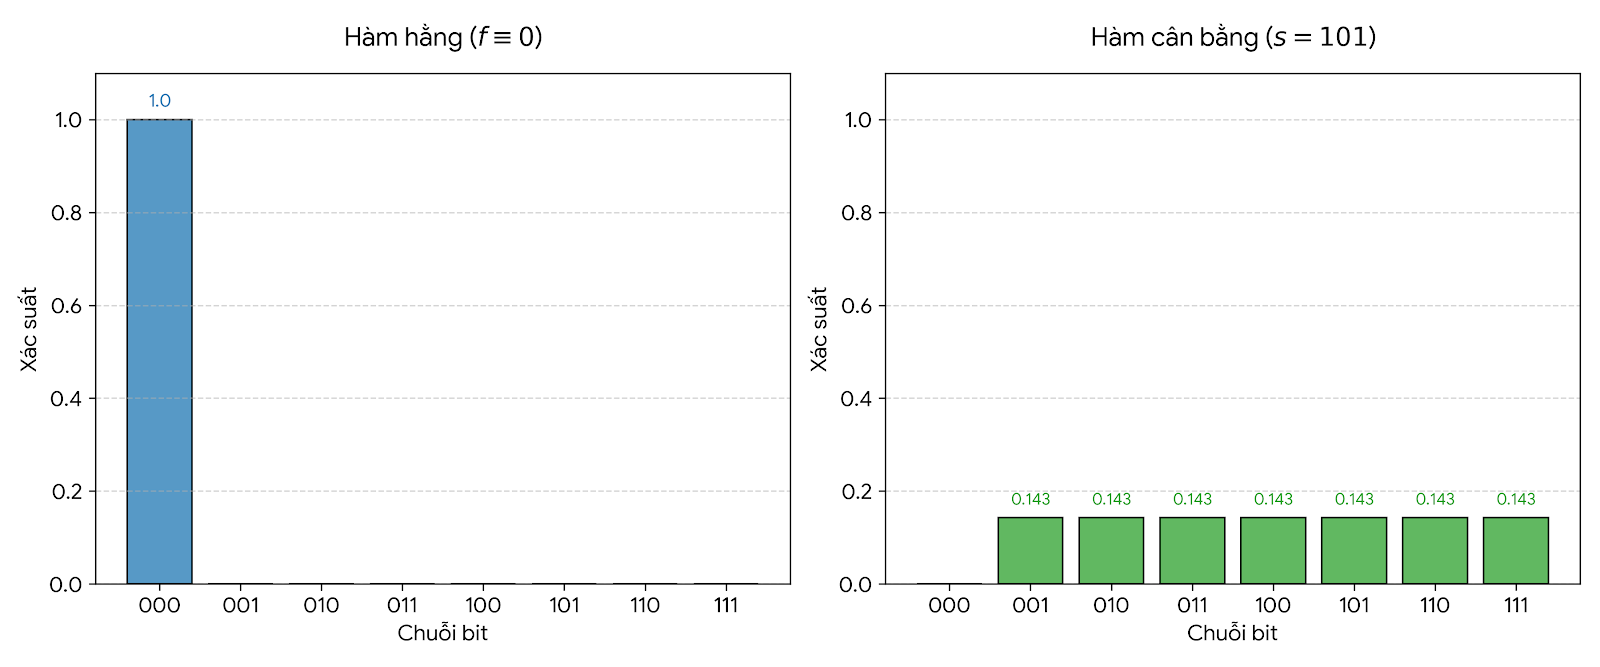
\includegraphics[width=1\textwidth]{assets/histogram.png}
    \caption{Biểu đồ xác suất đo của thuật toán Deutsch--Jozsa với $n=3$.}
    \label{fig:histogram-n3}
\end{figure}

Kết quả đầy đủ cho $n = 1, \ldots, 5$ được tổng hợp trong bảng sau.

\begin{table}[H]
\centering

\caption{Xác suất đo $P(|0\rangle^{\otimes n})$ của thuật toán Deutsch--Jozsa
         theo số qubit $n$}
\renewcommand{\arraystretch}{1.4}
\begin{tabular}{ccccc}
\hline
\multirow{2}{*}{$n$}
  & \multirow{2}{*}{Không gian ($2^n$)}
  & \multicolumn{2}{c}{$P(|0\rangle^{\otimes n})$}
  & \multirow{2}{*}{Kết luận} \\
\cline{3-4}
& & Hàm hằng & Hàm cân bằng & \\
\hline
$1$ & $2$  & $1.000$ & $0.000$ & Đúng \\
$2$ & $4$  & $1.000$ & $0.000$ & Đúng \\
$3$ & $8$  & $1.000$ & $0.000$ & Đúng \\
$4$ & $16$ & $1.000$ & $0.000$ & Đúng \\
$5$ & $32$ & $1.000$ & $0.000$ & Đúng \\
\hline
\end{tabular}

\end{table}

Kết quả trên cho thấy $P(|0\rangle^{\otimes n}) = 1$
với mọi hàm hằng và $P(|0\rangle^{\otimes n}) = 0$ với mọi hàm cân bằng,
bất kể $n$.

%────────────────────────────────────────────────────────────────────────────
\subsection*{So sánh với lý thuyết đã chứng minh}
%────────────────────────────────────────────────────────────────────────────

Kết quả mô phỏng xác nhận đầy đủ ba kết luận lý thuyết:

\textbf{(i) Tính đúng đắn tuyệt đối.} Với mọi $n$ từ $1$ đến $5$ và mọi
oracle thử nghiệm, thuật toán cho kết quả đúng với xác suất $1$ -- không
có trường hợp sai.

\textbf{(ii) Giao thoa tăng cường và triệt tiêu.} Toàn bộ xác suất tập trung tại
$|0\rangle^{\otimes n}$ (hàm hằng) hoặc hoàn toàn triệt tiêu tại đó (hàm
cân bằng).

\textbf{(iii) Tính độc lập với $n$.} Bảng 3.2 cho thấy kết
quả không phụ thuộc vào $n$: dù không gian trạng thái tăng từ $2^1 = 2$
lên $2^5 = 32$, thuật toán vẫn chỉ cần đúng một lần truy vấn oracle --
minh họa trực tiếp ưu thế $O(1)$ so với $O(2^{n-1})$ của thuật toán cổ
điển.

\subsection*{Kết luận cuối Chương 3}
Chương này đã hoàn thành mục tiêu trung tâm của khóa luận: phân tích
toán học đầy đủ và kiểm chứng thực nghiệm thuật toán Deutsch--Jozsa.
Bài toán được phát biểu chính xác, cơ chế phase kickback được chứng minh,
và kết quả trung tâm -- xác suất đo $P(|0\rangle^{\otimes n})$ bằng $1$
với hàm hằng và bằng $0$ với hàm cân bằng -- được thiết lập bằng chứng
minh toán học chặt chẽ. Ưu thế $O(1)$ so với $O(2^{n-1})$ của thuật toán
cổ điển được lý giải thông qua cơ chế giao thoa tăng cường và triệt tiêu,
và được xác nhận độc lập qua mô phỏng số với Qiskit cho $n = 1, \ldots, 5$.